\documentclass[twocolumn,10pt,a4paper]{article}
\usepackage[margin=0.75in]{geometry}
\usepackage[utf8]{inputenc}
\usepackage[T1]{fontenc}
\usepackage{lmodern}
\usepackage{microtype}
\usepackage{cite}
\usepackage{url}
\usepackage{hyperref}
\usepackage{xcolor}
\usepackage{enumitem}
\usepackage{tabularx}
\usepackage{booktabs}
\usepackage{graphicx}
\usepackage{tikz}
\usetikzlibrary{positioning,arrows.meta,fit,backgrounds,shadows}
\hypersetup{colorlinks=true,citecolor=blue,linkcolor=blue,urlcolor=blue}

\title{Paper 1: O2-IMS-to-Operator-CRD Runtime Architecture for Closed-Loop O-RAN Day-2 Remediation}

\author{David Kypuros \\
\small Red Hat \\
\small \texttt{dkypuros@redhat.com}}

\date{31 May 2026}

\begin{document}
\maketitle

\begin{abstract}
Paper 1 in this five-paper series describes the O2-IMS-to-operator-CRD runtime architecture for closed-loop O-RAN Day-2 remediation. The pattern composes standards and implementation contract layers: O-RAN O2 General Aspects and Principles (O2 GA\&P) for the O-Cloud resource model; O-RAN O2 Infrastructure Management Services (O2 IMS) as the SMO-to-O-Cloud infrastructure handoff; Kubernetes-native operator CRD surfaces (Metal3 BareMetal Operator (BMO) HostFirmwareComponents, Machine Config Operator (MCO) MachineConfig, and Kernel Module Management (KMM) Module resources) as the delivery substrate; TM Forum TMF688/TMF921-shaped audit and intent envelopes; and IEEE 1588 / O-RAN WG6 Cloud Notifications as the timing-domain observation contract. We claim the novelty lies in the O2-IMS-to-operator-CRD bridge: a deterministic routing rule classifies infrastructure faults against the O2 GA\&P O-Cloud resource model, hands the proposal through an O2-IMS-shaped handoff in v0, and represents delivery on existing Kubernetes operator contracts before any large language model is consulted. The contribution extends a prior multivendor diagnostic substrate by closing the loop from fault to audited remediation through a schema gate, a five-subcheck policy guardrail, and human co-authorization. The runtime is open-source and shipped with a verify gate that produces a binary pass/fail any reviewer can reproduce. We acknowledge that v0 runtime is stub-driven: it demonstrates an O2 IMS-shaped stub boundary and CRD-shaped fixtures, not live O2 IMS interop, live reconcile loops, or production wiring.
\end{abstract}

\section{Introduction}

Day-2 operations on a multivendor Cloud RAN deployment span a wide functional surface: timing drift on a worker node, firmware regressions on accelerator NICs, host service interference with the PTP hardware clock, driver swaps for fixed-function offloads, configuration churn from upstream SMO intents. Each of these is observable, each has an audited path to remediation, and yet the bridges between diagnosis and execution are uneven across vendors and standards bodies.

Prior agentic-AI work for RAN automation has clustered around two failure modes. The first stops at the SMO boundary: an agent converges on a root cause and emits an intent, but the intent never crosses into a concrete delivery contract. The second invents a parallel controller plane that side-steps O-RAN's own resource layering, which is operationally fragile and politically expensive in a multivendor ecosystem. A prior multivendor diagnostic publication established a fault-localization substrate for Cloud RAN troubleshooting \cite{multivendor_blog_2026} but left the loop open: the diagnostic agents converge on a root cause and emit an artifact, while the actual remediation path remains undefined.

This paper closes the loop. We describe a harness pattern that takes the diagnostic artifact as input, classifies it against a deterministic taxonomy grounded in the O-RAN O-Cloud resource model \cite{oran_wg1_arch,oran_o2_ganp}, routes the resulting proposal through an O2-IMS-shaped adapter boundary \cite{oran_o2_ims} toward Kubernetes-native CRD contracts (Metal3 BMO HostFirmwareComponents \cite{metal3_bmo} and MCO MachineConfig resources \cite{openshift_mco}, with KMM Module resources \cite{kmm_operator} as a third delivery path), and emits a TM Forum TMF688-shaped audit event \cite{tmf688} with a harness-specific reversibility profile before any apply is authorized. The four pieces (observation loop, cognitive middle, routing decision, sandbox plus operator seam) are described in order. We name the architectural novelty the \textbf{O2-IMS-to-operator-CRD bridge}: O2 GA\&P \cite{oran_o2_ganp} supplies the O-Cloud resource-layer model; O2 IMS \cite{oran_o2_ims} supplies the SMO-to-O-Cloud infrastructure handoff shape; Metal3 BMO \cite{metal3_bmo} supplies the bare-metal firmware and provisioning CRD path; and MCO \cite{openshift_mco} supplies the host-configuration CRD path. The taxonomy subtypes are harness-defined mappings into the O2 GA\&P Physical Resource, Logical Resource, and Managed O-Cloud Service classes; they are not proposed extensions to the O-RAN specification. The claim is not that any one interface is new. The claim is that their simultaneous composition lets a single \texttt{RemediationProposal} move from the runtime routing layer, through a standards-shaped O-RAN boundary, toward existing Kubernetes-native reconciler contracts without inventing a parallel controller plane. KMM is an extensibility witness within the same infrastructure route rather than part of the named four-element bridge.

The remainder of the paper is organized as follows. Section \ref{sec:background} establishes the standards and project context for each interface composed. Section \ref{sec:arch} describes the architecture in three logical pieces. Section \ref{sec:proto} summarizes the prototype, the five committed walkthrough scenarios, and the verify gate. Section \ref{sec:discuss} discusses positioning against adjacent projects and the standards-track ask. Section \ref{sec:conclude} concludes.

\section{Background}
\label{sec:background}

\textbf{O-RAN architecture and the O-Cloud surface.} The O-RAN Alliance Working Group 1 architecture description \cite{oran_wg1_arch} and Working Group 6 O2 General Aspects and Principles (O2 GA\&P) \cite{oran_o2_ganp} jointly define the O-Cloud resource model and the SMO-to-O-Cloud interface family. The O2 IMS specification \cite{oran_o2_ims} carries the infrastructure provisioning request and response envelopes; O2 DMS \cite{oran_o2_dms} carries deployment management. This work targets O2 IMS exclusively: the harness handles infrastructure remediation, not deployment lifecycle. The reference O2 IMS implementation cited throughout is Red Hat's open-source O-Cloud Manager \cite{oran_o2ims_ocm}. The Decoupled SMO Architecture technical report \cite{oran_decoupled_smo} introduces the SMO Service (SMOS) abstraction, into which a closed-loop remediation harness fits naturally as a candidate first-class SMOS.

\textbf{Delivery substrate.} Below the O2 IMS interface, three Kubernetes-native operators carry the actual change: the Machine Config Operator (MCO) reconciles MachineConfig resources for host configuration \cite{openshift_mco}, the Kernel Module Management Operator (KMM) reconciles Module resources for driver swaps \cite{kmm_operator}, and the Metal3 BareMetal Operator (Metal3 BMO) reconciles BareMetalHost and HostFirmwareComponents resources for bare-metal firmware and provisioning \cite{metal3_project,metal3_bmo}. Out-of-band firmware writes pass through the host BMC via DMTF Redfish \cite{dmtf_redfish}.

\textbf{Timing and observation.} The PTP stack on each worker uses linuxptp \cite{linuxptp_ptp4l} to discipline the PTP Hardware Clock (PHC) against an upstream Grandmaster, conforming to IEEE 1588-2019 \cite{ieee_1588_2019} and the ITU-T G.8275.1 telecom profile \cite{itu_g82751}. The Red Hat PTP Operator \cite{redhat_ptp_operator} orchestrates linuxptp on the cluster, and the cloud-event-proxy sidecar \cite{cloud_event_proxy} publishes state transitions as CloudEvents \cite{cncf_cloudevents} carrying the O-RAN WG6 Cloud Notifications payload \cite{oran_cloud_notifications}. The harness consumes that notification envelope as the inbound fault contract.

\textbf{Audit and intent.} TM Forum TMF688 \cite{tmf688} provides the event-management envelope used as the audit sink; the ReversibilityProfile carried here is harness-specific. TMF921 \cite{tmf921} provides the intent management envelope used for the dual-route notification path from the harness to the partner SMO; the \texttt{dispatch\_result} field is likewise harness-specific. The SID information framework \cite{tmf_gb922} grounds the conceptual model that maps O-RAN resource classes to TM Forum entity types.

\section{System Architecture}
\label{sec:arch}

\begin{figure*}[t]
\centering
\resizebox{0.98\textwidth}{!}{%
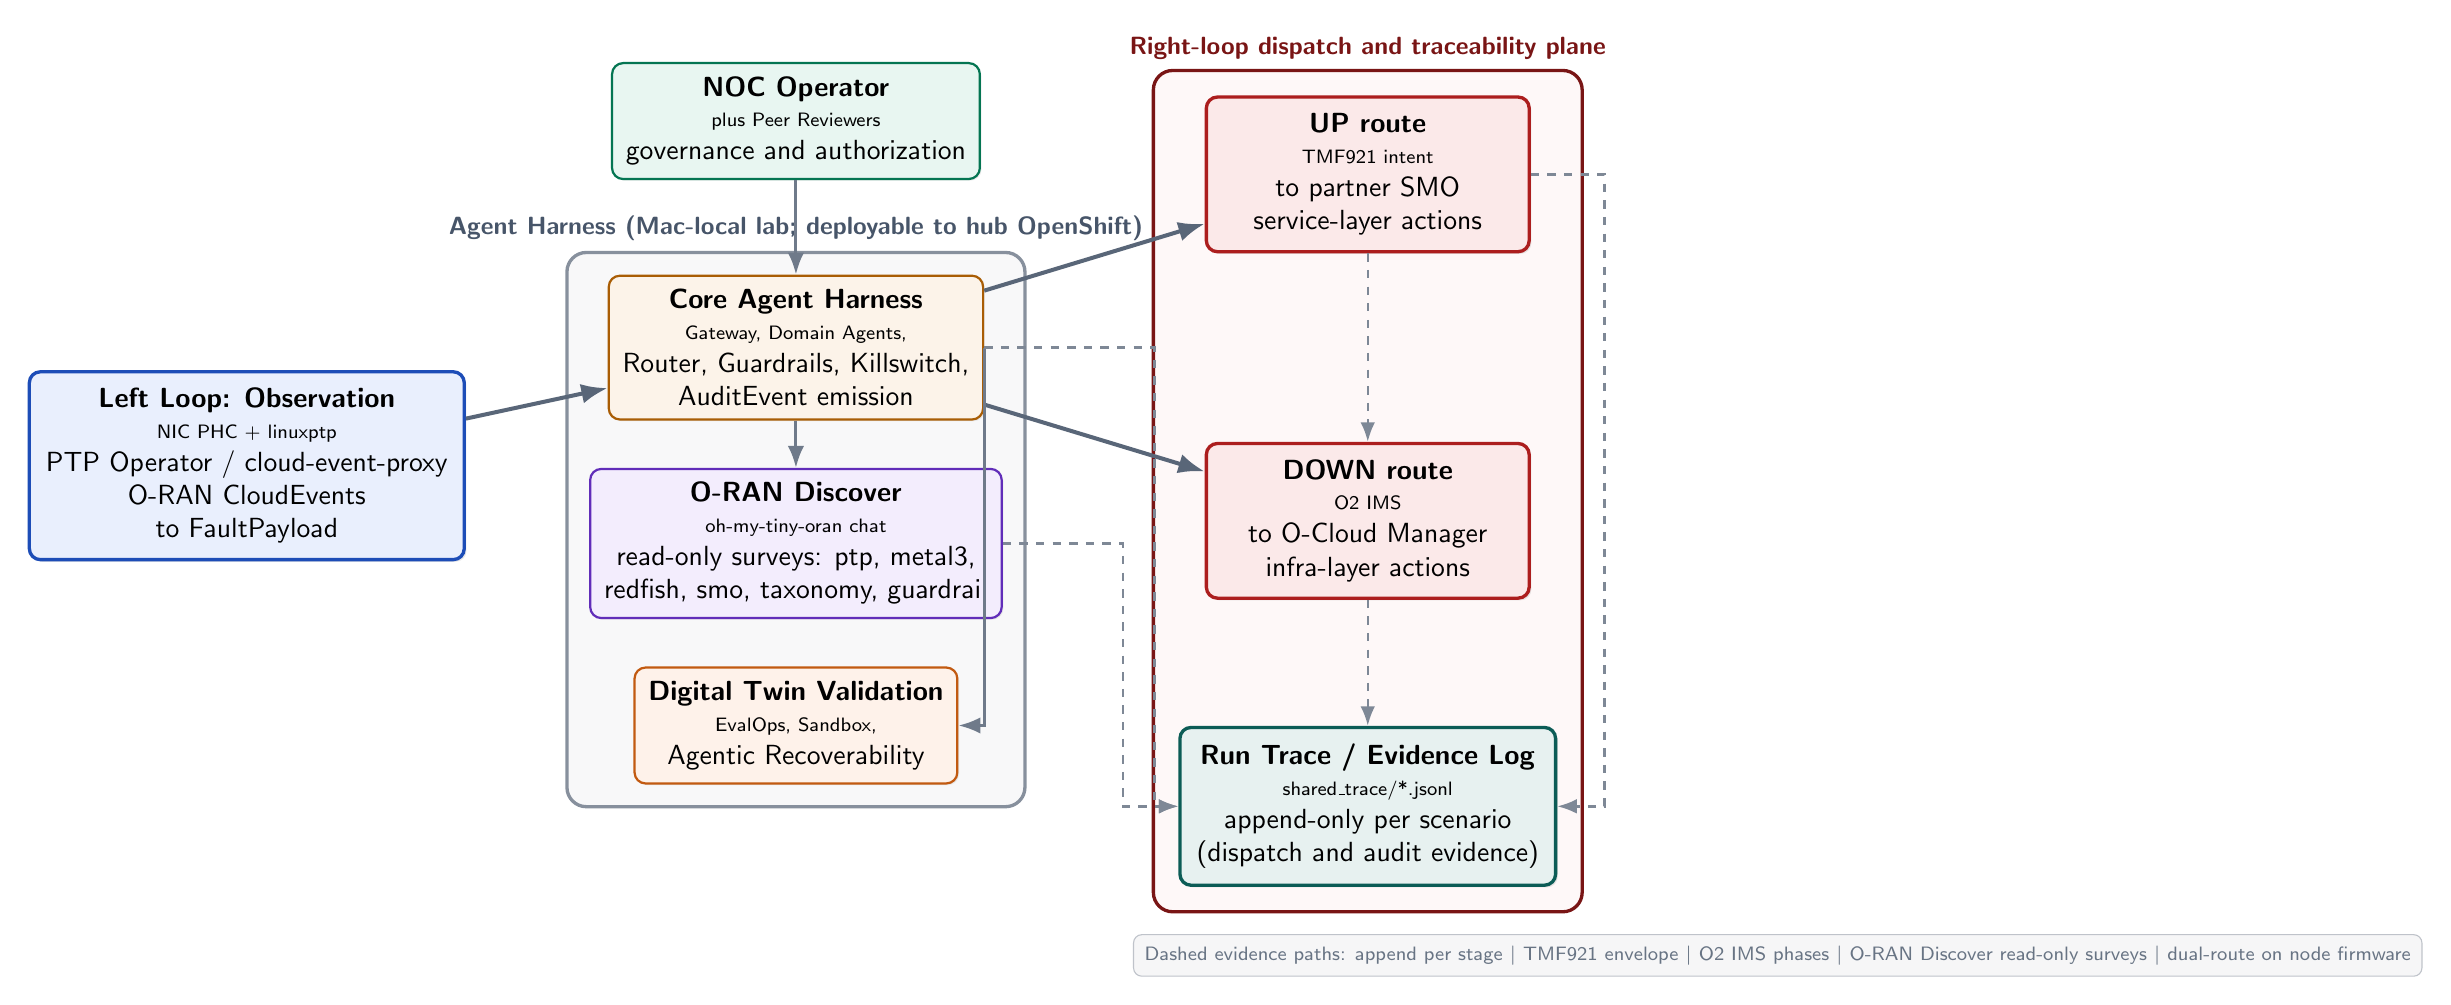
\begin{tikzpicture}[
  font=\sffamily,
  >=Latex,
  node distance=8mm and 12mm,
  macrobox/.style={
    draw=#1!78!black,
    fill=#1!10,
    very thick,
    rounded corners=4pt,
    align=center,
    minimum width=41mm,
    minimum height=18mm,
    inner sep=6pt,
    drop shadow={shadow xshift=0.8pt,shadow yshift=-0.8pt,opacity=0.18}
  },
  smallbox/.style={
    draw=#1!78!black,
    fill=#1!9,
    thick,
    rounded corners=4pt,
    align=center,
    minimum width=35mm,
    minimum height=13mm,
    inner sep=5pt,
    drop shadow={shadow xshift=0.6pt,shadow yshift=-0.6pt,opacity=0.14}
  },
  group/.style={
    draw=slate!65,
    fill=slate!4,
    rounded corners=7pt,
    very thick,
    inner sep=8pt
  },
  dispatchgroup/.style={
    draw=red!55!black,
    fill=red!3,
    rounded corners=7pt,
    very thick,
    inner sep=9pt
  },
  flow/.style={->,line width=1.1pt,draw=slate!78},
  strongflow/.style={->,line width=1.45pt,draw=slate!90},
  traceflow/.style={->,line width=0.9pt,draw=slate!70,dashed},
  note/.style={font=\scriptsize\sffamily,align=center,text=slate!80,fill=white,inner sep=2pt}
]
\definecolor{blue}{HTML}{2563EB}
\definecolor{amber}{HTML}{D97706}
\definecolor{green}{HTML}{059669}
\definecolor{rose}{HTML}{E11D48}
\definecolor{orange}{HTML}{F97316}
\definecolor{red}{HTML}{DC2626}
\definecolor{teal}{HTML}{0F766E}
\definecolor{purple}{HTML}{7C3AED}
\definecolor{slate}{HTML}{475569}

\node[macrobox=blue] (obs) {\textbf{Left Loop: Observation}\\[-1pt]
  \scriptsize NIC PHC + linuxptp\\PTP Operator / cloud-event-proxy\\O-RAN CloudEvents\\to FaultPayload};

\node[smallbox=amber, right=18mm of obs, yshift=15mm] (harness) {\textbf{Core Agent Harness}\\[-1pt]
  \scriptsize Gateway, Domain Agents,\\Router, Guardrails, Killswitch,\\AuditEvent emission};
\node[smallbox=purple, below=6mm of harness] (discover) {\textbf{O-RAN Discover}\\[-1pt]
  \scriptsize oh-my-tiny-oran chat\\read-only surveys: ptp, metal3,\\redfish, smo, taxonomy, guardrail};
\node[smallbox=orange, below=6mm of discover] (twin) {\textbf{Digital Twin Validation}\\[-1pt]\scriptsize EvalOps, Sandbox,\\Agentic Recoverability};
\node[smallbox=green, above=12mm of harness] (operator) {\textbf{NOC Operator}\\[-1pt]\scriptsize plus Peer Reviewers\\governance and authorization};

\begin{pgfonlayer}{background}
  \node[group, fit=(harness)(discover)(twin), label={[font=\bfseries\sffamily\small,text=slate]above:Agent Harness (Mac-local lab; deployable to hub OpenShift)}] (middle) {};
\end{pgfonlayer}

\node[macrobox=red, right=28mm of harness, yshift=22mm] (up) {\textbf{UP route}\\[-1pt]
  \scriptsize TMF921 intent\\to partner SMO\\service-layer actions};
\node[macrobox=red, right=28mm of harness, yshift=-22mm] (down) {\textbf{DOWN route}\\[-1pt]
  \scriptsize O2 IMS\\to O-Cloud Manager\\infra-layer actions};

\node[macrobox=teal, below=16mm of down] (trace) {\textbf{Run Trace / Evidence Log}\\[-1pt]
  \scriptsize shared\_trace/*.jsonl\\append-only per scenario\\(dispatch and audit evidence)};

\begin{pgfonlayer}{background}
  \node[dispatchgroup, fit=(up)(down)(trace), label={[font=\bfseries\sffamily\small,text=red!55!black]above:Right-loop dispatch and traceability plane}] (rightplane) {};
\end{pgfonlayer}

\draw[strongflow] (obs) -- (harness);
\draw[strongflow] (harness) -- (up);
\draw[strongflow] (harness) -- (down);
\draw[flow] (harness) -- (discover);
\draw[flow] (harness.east) |- (twin.east);
\draw[flow] (operator) -- (harness);

\draw[traceflow] (up.south) -- (down.north);
\draw[traceflow] (harness.east) -| ([xshift=-3mm]trace.west) -- (trace.west);
\draw[traceflow] (discover.east) -| ([xshift=-7mm]trace.west) -- (trace.west);
\draw[traceflow] (up.east) -| ([xshift=6mm]trace.east) -- (trace.east);
\draw[traceflow] (down.south) -- (trace.north);

\node[
  draw=slate!35,
  fill=slate!5,
  rounded corners=3pt,
  font=\scriptsize\sffamily,
  text=slate!82,
  align=center,
  below=6mm of trace.south east,
  xshift=28mm,
  minimum width=94mm,
  inner sep=4pt
] (legend) {Dashed evidence paths: append per stage $\vert$ TMF921 envelope $\vert$ O2 IMS phases $\vert$ O-RAN Discover read-only surveys $\vert$ dual-route on node firmware};
\end{tikzpicture}%
}
\caption{Seven-component macro architecture. The left loop is the observation loop: NIC PHC and linuxptp state are watched by the PTP Operator and cloud-event-proxy, emitted as O-RAN CloudEvents, and ingested as the harness \texttt{FaultPayload}. The NOC operator and peer reviewers sit above the harness as the governance and authorization layer. The Agent Harness contains the Agentic Gateway, MCP-backed domain agents, deterministic Router, guardrails, Killswitch, audit emission, O-RAN Discover read-only operator inspection surface, and Digital Twin validation substrate. The right side packages the service UP route, infrastructure DOWN route, and append-only run trace as one dispatch and traceability plane, so TMF921/O2 IMS handoffs and their evidence trail remain visually coupled.}
\label{fig:arch_macro}
\end{figure*}

The architecture has three logical pieces plus an explicit governance layer: the left loop (observation), the cognitive middle inside the Agent Harness, the right loop (routing, delivery, and traceability), and the NOC operator plus peer reviewers above the harness. The left loop is the observation loop under discussion here: bare-metal timing signals from the NIC PHC and linuxptp stack are carried by the PTP Operator and cloud-event-proxy into a CloudEvents-shaped \texttt{FaultPayload}. The Killswitch is a feature of the core harness guardrail path, and the Digital Twin is where validation takes place. Figure~\ref{fig:arch_macro} shows the macro layout.

\subsection{Left loop: observation}

Telemetry originates in the timing domain. Each Cloud RAN worker runs a PTP Hardware Clock disciplined by linuxptp daemons (\texttt{ptp4l} and \texttt{phc2sys}) \cite{linuxptp_ptp4l}, conforming to IEEE 1588-2019 \cite{ieee_1588_2019} and the G.8275.1 telecom profile \cite{itu_g82751}. The PTP Operator \cite{redhat_ptp_operator} runs the daemons and the cloud-event-proxy sidecar \cite{cloud_event_proxy} watches their state transitions. When the daemon state crosses a threshold (SYNCHRONIZED to HOLDOVER, master offset spike, monotonic PHC drift), the sidecar emits a CloudEvent \cite{cncf_cloudevents} with the O-RAN WG6 Cloud Notifications payload \cite{oran_cloud_notifications}.

The harness consumes this envelope as a \texttt{FaultPayload} (a JSON Schema draft-07 contract carried at \texttt{harness/schemas/FaultPayload.json}). The repository's scenario \texttt{D\_phc\_drift\_hw\_only} demonstrates the canonical divergence pattern that gives the harness its diagnostic edge: \texttt{ptp4l} reports SYNCHRONIZED (software view of the timing chain is healthy) while \texttt{phc2sys} reports monotonic frequency drift in parts-per-billion and the NIC reports rising \texttt{tx\_hwtstamp\_timeouts} (hardware view is not healthy). A purely software-layer observer would miss this; the harness reads both.

\subsection{Cognitive middle}

The Agentic Gateway terminates the CloudEvents stream and presents vendor-private tooling to the agent runtime under controlled MCP interfaces \cite{mcp_spec,mcp_python_sdk,fastmcp}. The v0 repository declares four MCP tool surfaces behind the gateway: \texttt{mcp-platform} (linuxptp daemons, host services, driver versions, NIC counters), \texttt{mcp-ran} (cell sync, PM counters, RAN parameters), \texttt{mcp-hardware} (NIC PHC introspection, BMC Redfish, CPU performance counters), and \texttt{mcp-ocloud} (the O-Cloud Manager inventory and alarms). A production deployment would run these as FastMCP servers with mTLS, OAuth2, and IP allowlists; the v0 lab treats the surfaces as local or stubbed and trusts localhost.

Three domain agents (Platform, RAN, Hardware) consume the MCP surface and converge on a root cause artifact (RCA). The cognitive middle's deterministic core is the Remediation Router. The router consults a 20-entry taxonomy declared in \texttt{harness/taxonomy.yaml}. Twelve infrastructure entries are grounded in O2 GA\&P Physical Resource, Logical Resource, or Managed O-Cloud Service classes; five service-layer entries are routed upward through TMF921; and three ambiguous entries require disambiguation before execution. The taxonomy carries an explicit grounding disclaimer in its first eighteen lines: the subtypes are interpretive mappings within, or deliberate layer-boundary separations from, the normative resource classes in O2 GA\&P Figure 3.4-1, not extensions to the spec.

The deterministic taxonomy lookup fires first; an LLM is consulted only when the result is the \texttt{ambiguous} class. This ordering is enforced in code and proven by the test suite. The repository's \texttt{contribution-1-routing-rule.yaml} declares the rule, the runtime at \texttt{harness/runtime/router.py} implements it, and the test \texttt{test\_route\_ambiguous\_with\_llm\_mode\_live} demonstrates that the LLM seam is wired through without becoming load-bearing on the routing decision. The live LLM test is support evidence for the seam, not part of the deterministic gate proof.

The LLM seam is provider-neutral: \texttt{completion()} can target Anthropic Claude, the OpenAI API, or an OpenAI-compatible on-premises vLLM endpoint such as Red Hat OpenShift AI \cite{litellm}. The MacBook dashboard can use \texttt{ANTHROPIC\_API\_KEY}, an OpenAI key, or an OpenAI-compatible local endpoint; the deterministic verify gate and the five committed scenarios do not depend on any hosted model.

\subsection{Right loop: routing and dual-route delivery}

The routing decision splits along the O-RAN resource-layer boundary. \textbf{Service-layer} faults (cell re-home, RAN parameter changes, slice intent updates, vDU software version rollouts) belong to the partner SMO. The harness does not execute them; it emits a TMF921-shaped companion intent \cite{tmf921} and observes the harness-specific dispatch result. This is the service route.

\textbf{Infrastructure-layer} faults go through the O2 IMS interface \cite{oran_o2_ganp,oran_o2_ims} into the O-Cloud Manager \cite{oran_o2ims_ocm}, which dispatches into one of three reconcilers: MCO \cite{openshift_mco} for host configuration changes, KMM \cite{kmm_operator} for driver swaps, and Metal3 BMO \cite{metal3_bmo} for node firmware. Firmware writes pass through the host BMC via DMTF Redfish UpdateService.SimpleUpdate \cite{dmtf_redfish}. This is the infrastructure route. In the v0 implementation, the infrastructure route is a real Python function call from the router into an O2 IMS-shaped stub boundary that returns a shape-correct \texttt{o2ims\_dispatch} envelope and points at committed CRD-shaped fixtures; the envelope is attached to the audit so the operator sees the intended O2 IMS hop as a row in the record, not as live interop or a synthesized path string.

The dual-route pattern fires both branches simultaneously when an infrastructure action carries inherent service-layer impact. Scenario \texttt{E\_nic\_firmware\_update} is the teaching case: a NIC firmware update via Metal3 BMO takes the host offline for a reboot window, so the harness emits a TMF921-shaped companion intent to the partner SMO in parallel with the O2 IMS infrastructure-route apply. The partner SMO's response (acceptance or rejection) lands on the audit's harness-specific \texttt{dispatch\_result} field before operator co-authorization. Scenario \texttt{E\_with\_smo\_reject} demonstrates the rejection path: same infrastructure-route verdict, SMO rejects the maintenance window because neighboring cells are at 92 percent capacity. The operator sees both outcomes and is the reconciliation point.

\subsection{Sandbox gate and reversibility}

Before any apply, the proposal traverses three deterministic control points: a JSON Schema gate, a five-subcheck policy guardrail declared at \texttt{harness/guardrails.yaml} and executed at \texttt{harness/runtime/guardrail.py}, and human co-authorization. The policy guardrail fires its subchecks in order: crisis\_mode global override, sandbox apply\_allowed, action\_allowlist, blast\_radius caps (one node, one site, four cells in v0), and requiresHumanApproval. The v0 runtime evaluates the sandbox subcheck against committed verdict fixtures; a production deployment would source that verdict from a same-topology mirrored cluster or a simulated linuxptp plus NIC driver stack.

Every TMF688-shaped audit event carries a populated harness-specific \texttt{ReversibilityProfile} with seven fields: rollback intent, blast-radius-if-reverse, rebuild timeline, replication history, validation history, risk profile burn-down, and confidence in reversibility. The intent is that the operator has the rollback contract at decision time, not after-the-fact. Figure~\ref{fig:governance} shows the governance layer in detail.

\begin{figure}[t]
\centering
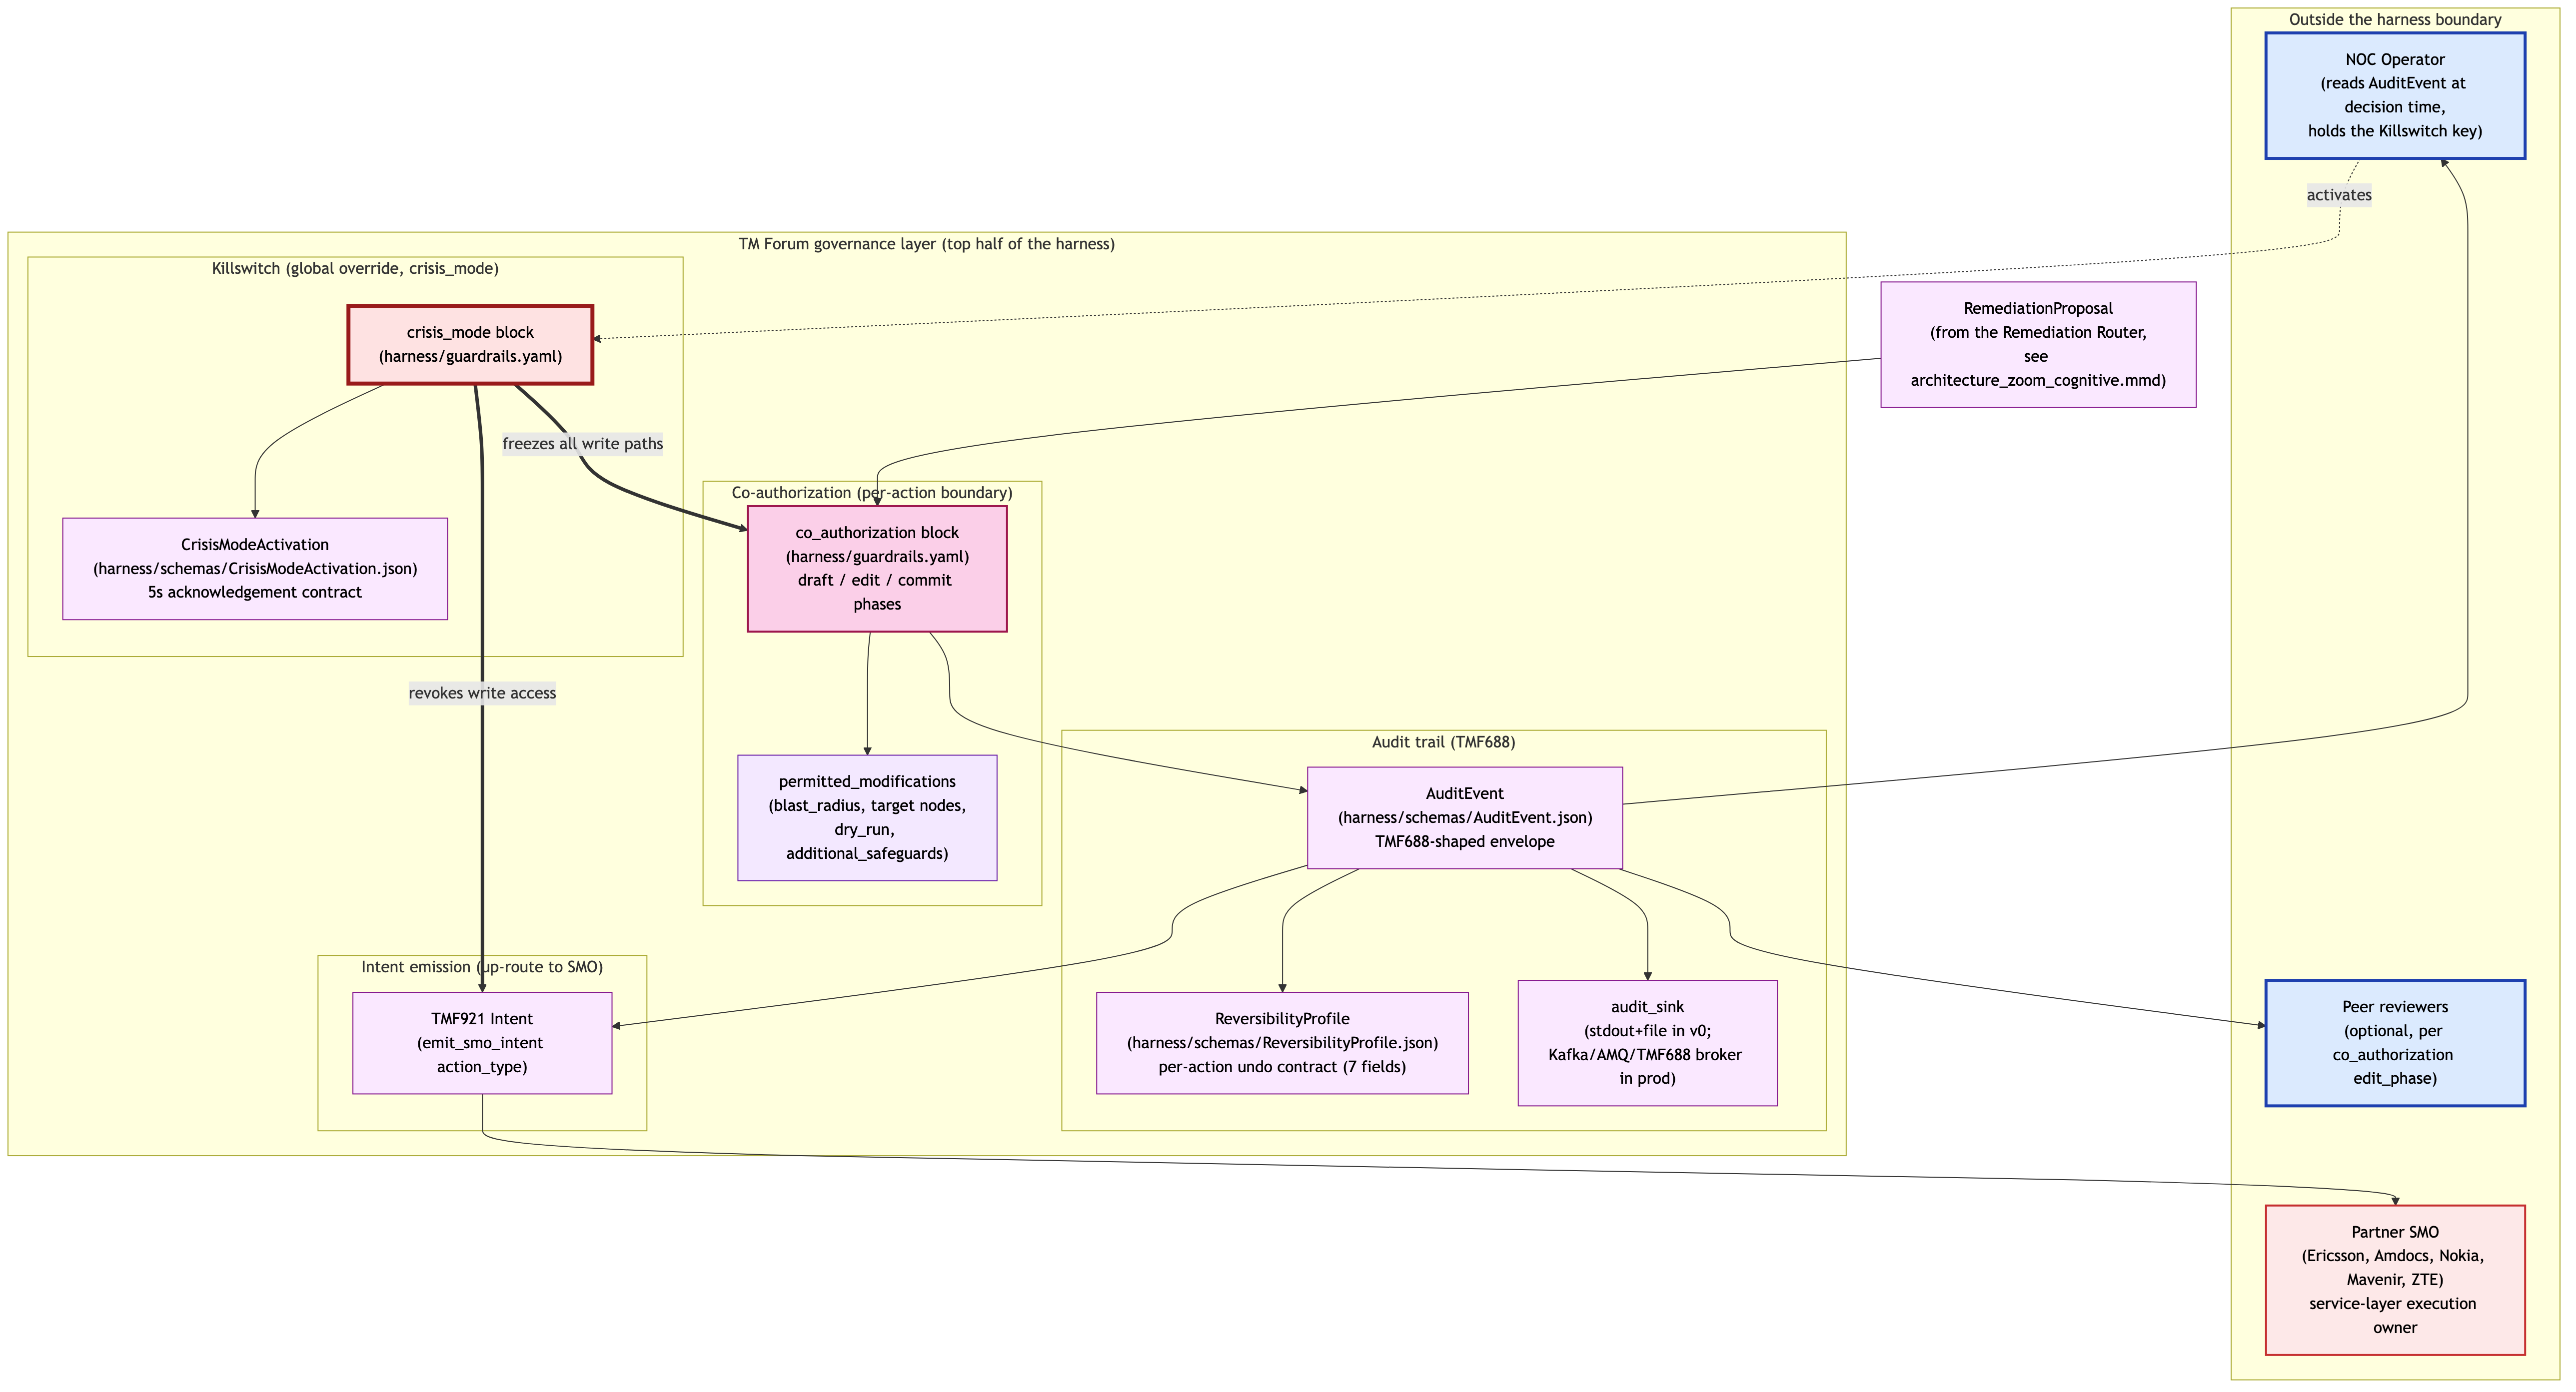
\includegraphics[width=\columnwidth]{../talk/architecture_zoom_governance.png}
\caption{Governance layer zoom. The TMF688-shaped audit event carries the proposal, the guardrail result, the sandbox verdict, the optional companion intent with its harness-specific dispatch result, and the seven-field ReversibilityProfile. The co-authorization contract sits between draft and commit. The Killswitch (crisis\_mode) is the global override.}
\label{fig:governance}
\end{figure}

\subsection{Killswitch as global override}

A \texttt{crisis\_mode} flag in \texttt{guardrails.yaml} is the global override. When activated by a NOC supervisor in response to a macro event (storms, security incidents, regional outages), all write paths revoke, EvalOps confidence pins to zero, and telemetry routes to a manual queue. The Reversibility Profile rewinds one applied action; the Killswitch freezes all of them. The two compose.

\subsection{Operator-facing discovery surface}

The MacBook lab exposes the cognitive middle through \texttt{oh-my-tiny-oran}, a small OMC-shaped chat harness scoped to the read-only \texttt{oran-discover} bundle at \texttt{omc-skills/oran-discover/}. The chat service inlines the invoked skill markdown into the turn and permits only bounded reads: HTTP GET calls against lab wrappers and reads from committed repository files. The seven operator skills are therefore cognitive scaffolding, not remediation machinery. Six probes inspect one surface each, and \texttt{/oran-discover:plan} composes them as a pre-flight walk before the operator considers any write-capable workflow.

The reviewer-facing right-loop demo deliberately keeps two surfaces separate. The \texttt{/commands} and \texttt{/oran-discover:*} paths are read-only inspection surfaces for PTP, Metal3, Redfish, SMO, taxonomy, and guardrail state. The \texttt{harness-walker} \texttt{/run/\{scenario\}} path is a separate deterministic sidecar that returns the \texttt{AuditEvent}; the chat assistant may inspect or explain that event, but it does not become the router, guardrail, or approval authority.

\begin{table*}[t]
\centering
\scriptsize
\begin{tabularx}{\textwidth}{p{3.8cm}p{3.2cm}X}
\toprule
Skill & Primary harness surface & Read path summarized for the operator \\
\midrule
\texttt{/oran-discover:ptp} & Left-loop observation & PTP sync state, PHC drift, linuxptp state, and CloudEvents / O-RAN Cloud Notifications wrapper output. \\
\texttt{/oran-discover:metal3} & Infrastructure route & Metal3 BMO BareMetalHost and HostFirmwareComponents state behind the O2 IMS shaped handoff. \\
\texttt{/oran-discover:redfish} & Hardware and BMC substrate & Redfish BMC task state, cross-checked against the Metal3 firmware path rather than exposed as a direct write path. \\
\texttt{/oran-discover:smo} & Service route & TMF921-shaped companion intent state and the partner-SMO response surface used by dual-route cases. \\
\texttt{/oran-discover:taxonomy} & Cognitive middle & The 20-entry routing taxonomy, including infrastructure, service, and ambiguous layer-boundary classes. \\
\texttt{/oran-discover:guardrail} & Governance overlay & The deterministic policy state: allowlist, blast-radius caps, \texttt{requiresHumanApproval}, and \texttt{crisis\_mode}. \\
\texttt{/oran-discover:plan} & Pre-flight orchestration & A read-only walk across the six probes so the operator can inspect evidence, routing, and policy before authorization. \\
\bottomrule
\end{tabularx}
\caption{The \texttt{oran-discover} operator skills. They expose the left loop, cognitive middle, right-loop service and infrastructure state, and governance overlay as read-only inspection surfaces.}
\label{tab:discover-skills}
\end{table*}

\section{Prototype and Walkthroughs}
\label{sec:proto}

\begin{figure}[t]
\centering
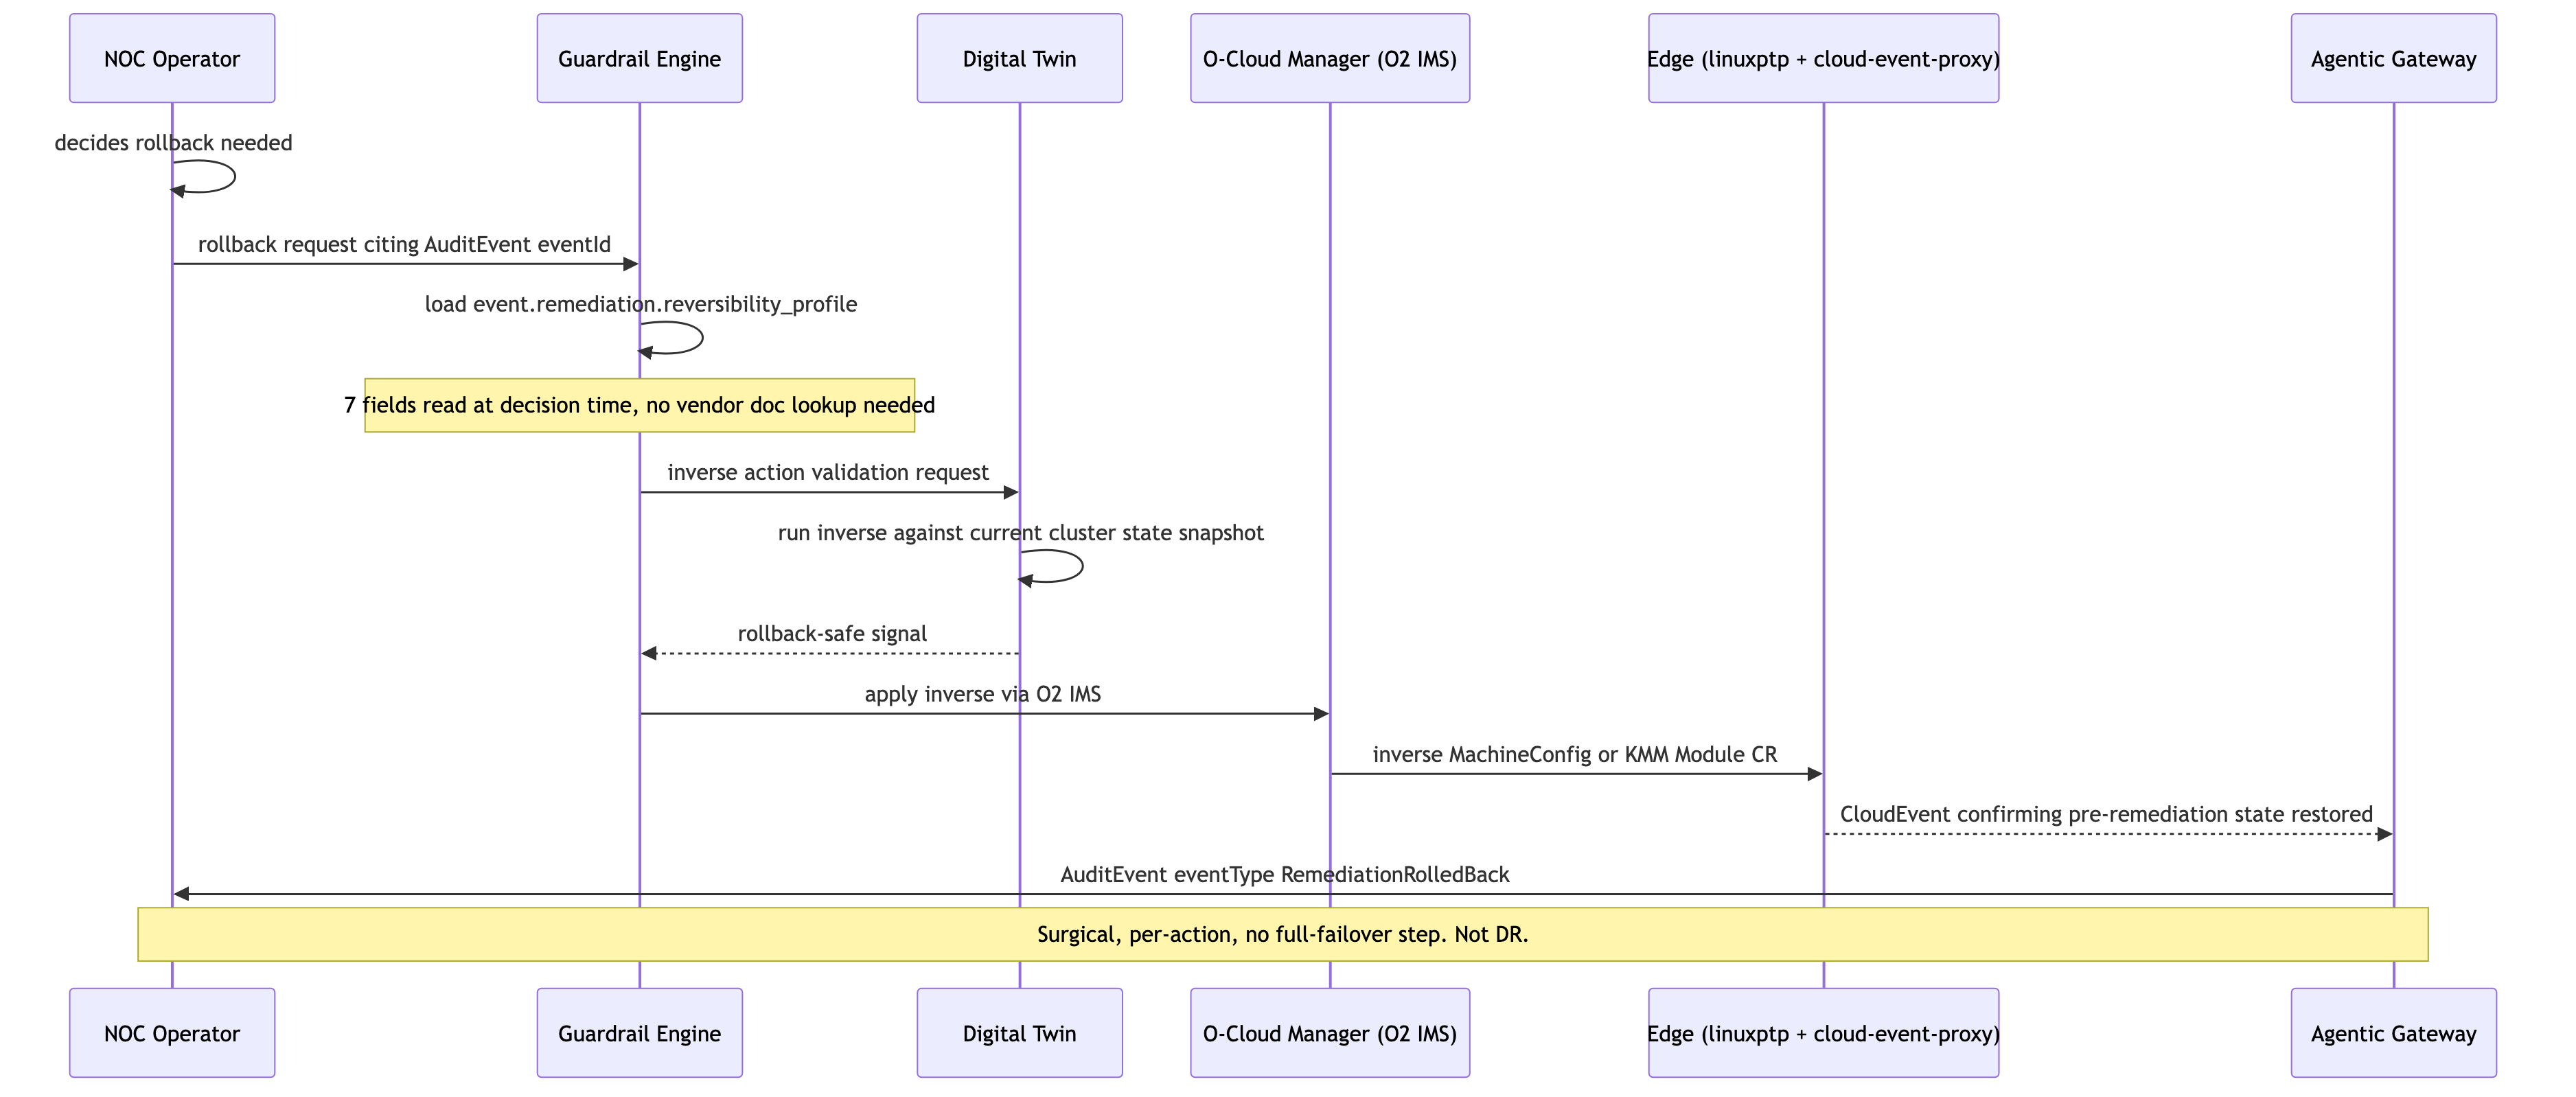
\includegraphics[width=\columnwidth]{../talk/sequence_agentic_recovery.png}
\caption{Sequence diagram for a single closed-loop remediation cycle. PTP CloudEvent arrives at the gateway, traverses the runtime router to a RemediationProposal, passes the schema gate and five-subcheck policy guardrail, lands on the operator's human co-authorization seat, and emits a TMF688-shaped audit event with the harness-specific reversibility profile attached.}
\label{fig:sequence}
\end{figure}

The repository ships five end-to-end fixture scenarios under \texttt{scenarios/}: \texttt{A\_fw\_lldp\_agent} (a host service interfering with PTP, routed to MCO), \texttt{A\_prime\_ice\_driver} (an outdated NIC driver causing PHC drift, routed to KMM), \texttt{D\_phc\_drift\_hw\_only} (the hardware-only divergence demonstrating the diagnostic edge), \texttt{E\_nic\_firmware\_update} (the dual-route firmware case with accepted companion intent), and \texttt{E\_with\_smo\_reject} (the same firmware path with a rejected companion intent). Each scenario carries a \texttt{fault\_payload.json} input, a remediation YAML, and a committed \texttt{audit\_event.json} fixture that the verify gate replays against the actual walker output.

The empirically exercised MacBook/Sheldon walkthrough makes three right-loop branches visible without expanding the v0 interop claim. In \texttt{D\_phc\_drift\_hw\_only}, the taxonomy selects \texttt{host\_driver} and the down route is O2 IMS to the O-Cloud KMM driver path. In \texttt{E\_nic\_firmware\_update}, the taxonomy selects \texttt{node\_firmware}; the harness shows the O2 IMS down route toward Metal3/Redfish and the TMF921 companion intent up route toward the SMO. In \texttt{E\_with\_smo\_reject}, the same infrastructure route remains shape-correct while the SMO companion dispatch is rejected before human co-authorization, leaving the operator as the reconciliation point. In all three branches the endpoints are stubs, but the routing decision, guardrail result, sandbox verdict, \texttt{AuditEvent}, and chat/sidecar wiring are real harness behavior.

The v0 runtime pipeline (walker, router, sandbox-fixture evaluation, guardrail) is deterministic. A reviewer can clone the repository, install PyYAML and jsonschema, and run \texttt{python3 scripts/verify.py}. With jsonschema installed, the gate completes ten checks in under five seconds: citation header completeness on every authored YAML and JSON, JSON and YAML parse, traceability-table bidirectional completeness, an em-dash audit, a leakage guard, README structural sanity, file counts, JSON Schema validation of every scenario fault payload plus the embedded remediation and reversibility-profile subobjects, and end-to-end walker replay against committed audit fixtures on eight material comparisons (seven named fields plus the reversibility profile confidence sub-field). In reduced environments where jsonschema is absent, check 9 is reported as skipped and the reduced gate reports the executed checks.

\section{Discussion}
\label{sec:discuss}

\textbf{The O2-IMS-to-operator-CRD bridge.} The architecture's central claim is that a single \texttt{RemediationProposal} travels through the O2 GA\&P resource model and an O2 IMS contract surface \cite{oran_o2_ganp,oran_o2_ims}, then is represented at an existing Kubernetes-native operator CRD reconciler such as Metal3 BMO or MCO \cite{metal3_bmo,openshift_mco} without a custom controller plane in between. In v0, this is demonstrated as fixture replay over a shape-correct O2 IMS stub plus committed CRD-shaped fixtures, not live O2 IMS interop. The conjunction of O2 GA\&P, O2 IMS, Metal3 BMO, and MCO is not a re-derivation of prior architectures; existing agentic-RAN work either stops at the SMO boundary without a delivery story, or proposes a parallel controller plane. The harness pattern composes existing contracts.

\textbf{Comparison to ONAP, Nephio, OSM.} ONAP \cite{onap}, Nephio \cite{nephio}, and Open Source MANO \cite{osm} are orchestration platforms that manage network function lifecycle at scale. The harness pattern is closed-loop remediation: fault-driven cognition that emits a proposal, gates it, audits it, and observes the operator's commit. The two compose. Nephio can deliver the standing topology; the harness handles post-deployment Day-2 anomalies on top of that topology.

\textbf{Positioning against the Decoupled SMO Architecture.} The closed-loop harness fits the SMOS abstraction described in WG1 TR R004 \cite{oran_decoupled_smo}. It exposes a TMF688-shaped audit surface and a TMF921-shaped intent surface as a candidate SMOS-compatible interface shape (interop testing against an SMOS-conformant catalogue is a v1 work item). A reasonable standards-track ask is for an nGRG output that names a Closed-Loop Remediation SMOS as a first-class element of the Decoupled SMO catalogue, and a TM Forum Implementation Guide companion that documents two harness-unique extensions as candidate API additions: a \texttt{dispatch\_result} field on the TMF921 companion intent envelope, and the seven-field ReversibilityProfile attached to every TMF688-shaped audit event.

\textbf{Layer-boundary discipline.} The harness is explicit about what it does not target. O-RAN R1 \cite{oran_r1} is the SMO-internal service-exposure interface for rApps; the harness's MCP gateway is internal agent scaffolding, not R1. A1 \cite{oran_a1} targets Near-RT RIC behavior (slice SLA, traffic steering); the harness targets the infrastructure layer below. E2 \cite{oran_e2} governs Near-RT RIC interactions with O-CU and O-DU; the harness does not consume E2 directly. O1 \cite{oran_o1} governs SMO-to-managed-element OAM; the harness operates below the managed-element boundary because the O-Cloud is platform, not managed element. These disclaimers are not modesty; they preserve the composability claim.

\textbf{Honest-scope acknowledgements.} The v0 runtime is stub-driven for the five committed scenarios. The platform stubs at \texttt{5G\_O-RAN\_SIM/oam/} emit shape-correct envelopes without crossing real network boundaries. The five-subcheck policy guardrail enforces v0 absolute limits (one node, one site, four cells); a production deployment would wire to a policy-as-code system (OPA or Kyverno) and source limits from a service catalog. Multi-cluster scale is not demonstrated. The co-authorization edit-phase (operator amending the proposal before commit instead of approving or rejecting it) is the v1 target; v0 enforces a boolean approval gate.

\section{Conclusion}
\label{sec:conclude}

This paper has described a closed-loop Day-2 remediation harness pattern for O-RAN Cloud RAN deployments. The pattern composes pre-existing standardized and implementation contracts (O2 GA\&P, O-RAN O2 IMS, Kubernetes-native operator CRDs, TM Forum TMF688 and TMF921, IEEE 1588 plus O-RAN Cloud Notifications) under a deterministic routing rule grounded in the O-RAN WG6 O-Cloud resource model. The O2-IMS-to-operator-CRD bridge, O2 GA\&P plus O2 IMS plus Metal3 BMO plus MCO, is the architectural novelty, with KMM as an additional co-delivery path. The runtime is open-source, exercised end-to-end by a fixture-driven verify gate, and ships with five walkthrough scenarios including a dual-route firmware case with both accepted and SMO-rejected variants. v0 limits are declared in code and in this paper: fixture replay demonstrates an O2 IMS-shaped stub boundary and CRD-shaped fixtures, not live O2 IMS interop, live reconcile loops, or production interop.

\section*{Acknowledgements}

This work extends a prior multivendor diagnostic substrate published as an Ericsson Technology Blog and co-authored with S. Kiani Mehr, N. Korati Prasanna, M. Vazquez Cebrian, S. Srikanthan, and P. Venkatesh \cite{multivendor_blog_2026}. Killswitch design feedback was received from operator stakeholders. Apache-2.0 licensed source code: \url{https://github.com/dkypuros/oran-agent-harness}.

\bibliographystyle{plain}
\bibliography{refs}

\end{document}
